\section{590 --- N-ary Tree Postorder Traversal}
Given an $n$-ary tree, return the \textit{postorder} traversal of its nodes' values.

For example, given a 3-ary tree:

\begin{figure}[H]
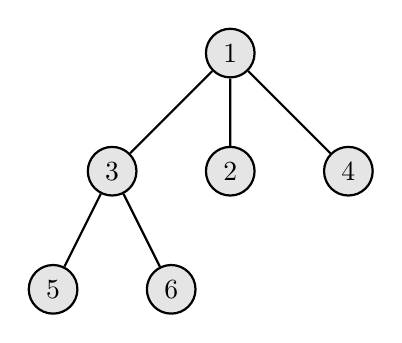
\begin{tikzpicture}
[every node/.style={draw, circle,minimum size=6mm, fill=gray!20!}, node distance=8mm,thick]
\node{1}
child{node{3} child{node{5}} child{node{6}}}
child{node{2}}
child{node{4}};
\end{tikzpicture}
\end{figure}

Return its postorder traversal as: $[5,6,3,2,4,1]$.


\paragraph{Note:}

\begin{itemize}
\item Recursive solution is trivial, could you do it iteratively?
\end{itemize}

\subsection{Stack}
\begin{itemize}
\item Similar to binary tree preorder traverse, we make use of a stack.
\item First, push the root into the stack.
\item At each iteration, pop the top node from the stack, add the value to the output and then push its children from start to end to the stack. 
\item Finally, we need to reverse the output.
\end{itemize}

\setcounter{lstlisting}{0}
\begin{lstlisting}[style=customc, caption={Stack}]
vector<int> postorder( Node* root )
{
    if( !root )
    {
        return {};
    }

    stack<Node*> stk;

    stk.push( root );

    vector<int> ans;

    while( !stk.empty() )
    {
        auto t = stk.top();
        stk.pop();
        ans.push_back( t->val );

        for( auto node : t->children )
        {
            //push the children sequentially
            stk.push( node );
        }
    }

    //we have to reverse the output
    reverse( begin( ans ), end( ans ) );

    return ans;
}
\end{lstlisting}